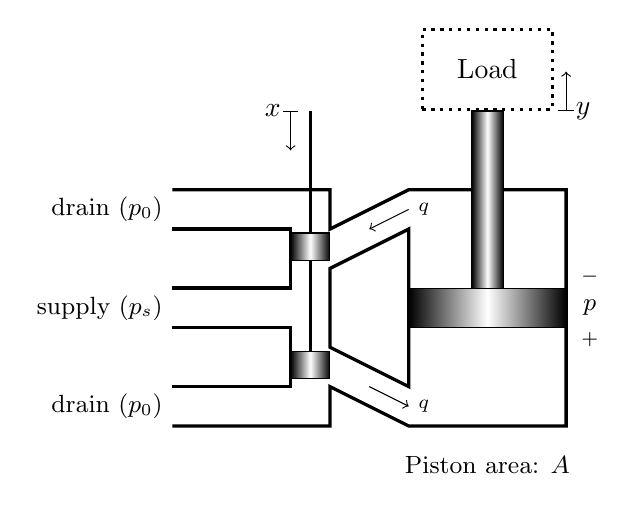
\begin{tikzpicture}

% tank
\draw[very thick] (0,0) -- ++(2,0) -- ++(0,-.5) -- ++(1,.5) -- ++(2,0) -- ++(0,-3) -- ++(-2,0) -- ++(-1,.5) -- ++(0,-.5) -- ++(-2,0);
\draw[very thick] (0,-.5) -- ++(1.5,0) -- ++(0,-.75) -- ++(-1.5,0);
\draw[very thick] (0,-1.75) -- ++(1.5,0) -- ++(0,-.75) -- ++(-1.5,0);
\draw[very thick] (2,-1) -- ++(1,.5) -- ++(0,-2) -- ++(-1,.5) -- cycle;
\draw (4,-3.5) node {\small Piston area: $A$};
\draw (0,-.25) node[left] {\small drain ($p_{0}$)};
\draw (0,-1.5) node[left] {\small supply ($p_{s}$)};
\draw (0,-2.75) node[left] {\small drain ($p_{0}$)};
\draw[->] (3,-.25) node[right] {\scriptsize$q$} -- ++(-.5,-.25);
\draw[->] (2.5,-2.5) -- ++(.5,-.25)  node[right] {\scriptsize$q$};
\draw (5.3,-1.9) node {\scriptsize $+$} ++(0,.4) node{\small $p$} ++(0,.4) node {\scriptsize$-$};

% valves
\draw[very thick,color=black] (1.75,-2.1) -- ++(0,3.1);
\draw[fill,left color=black,right color=black,middle color=white] (1.5,-.9) rectangle ++(.5,.35);
\draw[fill,left color=black,right color=black,middle color=white] (1.5,-2.4) rectangle ++(.5,.35);
\draw[|->] (1.5,1) node[left] {$x$} -- ++(0,-.5); 

% piston
\draw[fill,left color=black,right color=black,middle color=white] (4,-1.5) ++(-.2,0) rectangle ++(.4,2.5);
\draw[fill,left color=black,right color=black,middle color=white] (3,-1.75) rectangle ++(2,.5);
\draw[|->] (5,1) node[right] {$y$} -- ++(0,.5);

% load
\draw (4,1) node[draw,very thick,above,dotted,rectangle,minimum width=.65in,minimum height=.4in] {Load};

%% regulator
%\draw[fill] (2.5,1.5) circle (3pt);
%\draw[thick] (1.75,1.5) -- (4,1.5);
\end{tikzpicture}